
\tikzstyle{block} = [draw, fill=blue!20, rectangle,
    minimum height=3em, minimum width=4em]
\tikzstyle{sum} = [draw, fill=blue!20, circle, node distance=1cm]
\tikzstyle{input} = [coordinate]
\tikzstyle{output} = [coordinate]
\tikzstyle{out} = [coordinate]
\tikzstyle{pinstyle} = [pin edge={to-,thin,black}]
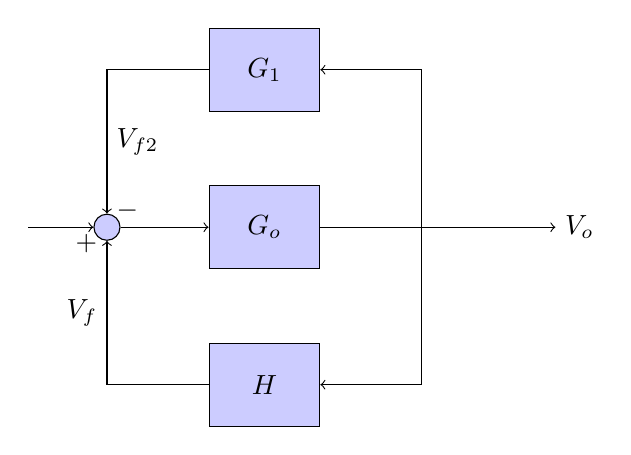
\begin{tikzpicture}[auto, node distance=2cm]
    \node [input, name=input] {};
    \node [sum, right of=input] (sum) {};
    \node [block, right of=sum] (controller) {$G_o$};
    \node [block, above of= controller](feedback2){$G_1$};
    \node [output, right of=controller] (output) {};
    \node [right of=output](out){$V_{o}$};
    \node [block, below of=controller] (feedback) {$H$};
    \draw [draw,->] (input) -- node {} (sum);
    \draw [->] (sum) -- node {} (controller);
    \draw [-] (controller) -- node {}(output);
    \draw [->] (output) |- (feedback);
    \draw [->] (output) |- (feedback2);
     \draw [->] (output) |- node{}(out);
     \draw [->] (feedback2) -| node[pos=0.99]{$-$}  node [near end] {$V_{f2}$} (sum);
    \draw [->] (feedback) -| node[pos=0.99]{$+$}  node [near end] {$V_f$} (sum);
\end{tikzpicture}
